

The lower-right plot in Figure~\ref{helicityDistDataMCnoLDcut} shows a discrepancy at low LD values.
To identify the source of this discrepancy and quantify the impact on the signal, we have studied
the distributions of the helicity angles before the LD cut. The overall agreement is very good in
all the angles, except in the $\cos\theta^\ast$ distribution for Z+jets events at
$|\cos\theta^\ast| > 0.85$. As a cross-check, Figure~\ref{fig:ctsarcut} presents the LD distribution
applying the cut $|\cos\theta^\ast| < 0.85$, compared to the original LD distribution.
After this cut, Z+jets events are rejected with a minimal impact on the signal efficiency, less than 0.5\%,
and the agreement of the MC with data is significantly improved. 

As an alternative cross-check, rather than cutting in $|\cos\theta^\ast|$, we have weigthed the Z+jets MC
to correct for the improper behavior at $|\cos\theta^\ast| > 0.85$. The resulting distributions 
of $\cos\theta^\ast$ and LD, displayed in Figure~\ref{fig:newldplots}, show a good agreement of the MC
with data, in particular in the LD distribution.

This study demonstrates that the disagreement at low LD values is due to a bad modeling of the
$\cos\theta^\ast$ distribution of Z+jets events at $|\cos\theta^\ast| > 0.85$,
which has a negligible impact on the signal, giving confidence in the analysis.
%%%%%%%%%
\begin{figure}[h]
\centering
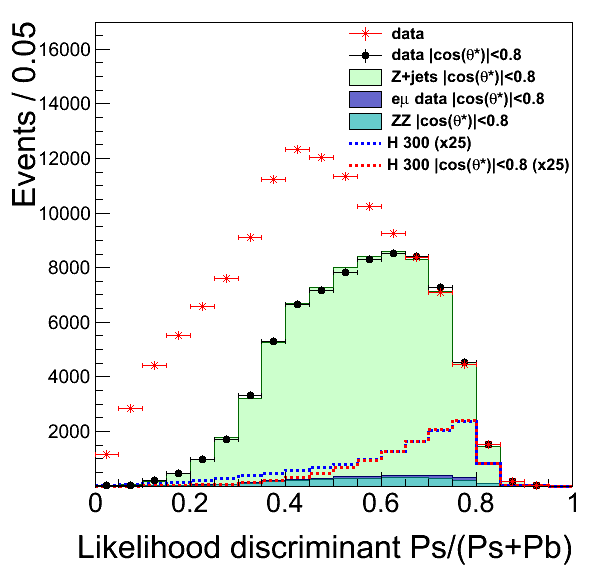
\includegraphics[width=0.49\textwidth]{plots/LD_CUT_ctSTAR.png}
\caption{LD distribution for data (black dots), background (coloured histrograms), and
signal (dashed red line, $\times 25$) events that pass the cut  $|\cos\theta^\ast| < 0.85$.
Uncut distributions for data (red dots) and signal (dashed blue line, $\times 25$) are also
displayed for comparison.
}
\label{fig:ctsarcut}
\end{figure}

\begin{figure}[h]
\centering
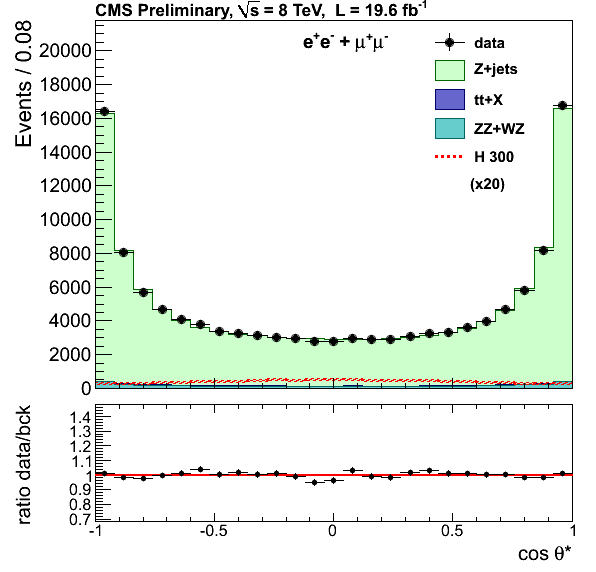
\includegraphics[width=0.49\textwidth]{plots/h_ll_cts_weighted.png}
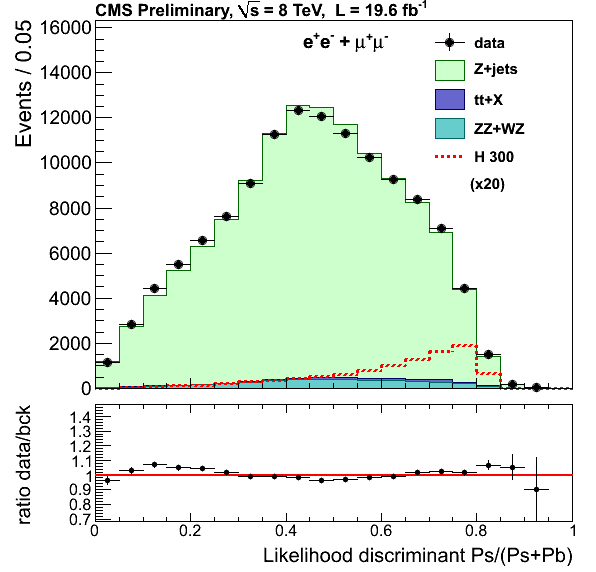
\includegraphics[width=0.49\textwidth]{plots/h_ll_ld_weighted.png}
\caption{$\cos\theta^\ast$ and LD distributionis for data (balck dots), background (coloured histrograms), and
signal (dashed red line, $\times 20$) events. The Z+jets MC is weighted to match the $\cos\theta^\ast$
distribution in data.
}
\label{fig:newldplots}
\end{figure}
